\documentclass[twocolumn, 10pt]{article}

% ── XeLaTeX Font Stack (COMPILE WITH XeLaTeX, NOT pdfLaTeX) ──
\usepackage{fontspec}
\setmainfont{TeX Gyre Termes}[
  Ligatures      = TeX,
  BoldFont       = {TeX Gyre Termes Bold},
  ItalicFont     = {TeX Gyre Termes Italic},
  BoldItalicFont = {TeX Gyre Termes Bold Italic},
]
\usepackage{unicode-math}
\setmathfont{TeX Gyre Termes Math}

% ── Packages ──
\usepackage{amsmath, amssymb}
\usepackage{graphicx}
\usepackage{booktabs}
\usepackage{hyperref}
\usepackage{float}
\usepackage[margin=0.85in]{geometry}
\usepackage{caption}
\usepackage{enumitem}
\usepackage{microtype}

% ── Metadata ──
\title{\textbf{Eccentricity-Driven Error Scaling in the Kepler Problem:\\ Quantifying the Energy Drift Rates of Numerical Integrators}}
\author{Mosin Mushtaq}
\date{March 2026}

\begin{document}
\maketitle

% ================================================================
% ABSTRACT
% ================================================================
\begin{abstract}
The secular growth of energy error in numerical integration of the unperturbed Kepler two-body problem was investigated as a function of orbital eccentricity~$e$. Three integration schemes---the Forward Euler method, the Classical Runge-Kutta method (RK4), and the Velocity Verlet method (symplectic)---were applied to 100-orbit simulations across $e \in [0.1,\, 0.7]$ with strict 64-bit floating-point arithmetic. The fractional energy error was found to obey a power-law scaling $|\Delta E / E_0| \propto (1 - e)^{-k}$, with the exponent~$k$ serving as a quantitative fingerprint of eccentricity sensitivity. RK4 exhibited the steepest scaling ($k = 8.61 \pm 0.03$), Verlet showed intermediate sensitivity with bounded oscillations ($k = 4.88 \pm 0.02$), and Euler displayed the weakest eccentricity dependence ($k = 0.44 \pm 0.09$) despite accumulating the largest absolute errors. A time-step robustness validation confirmed that the RK4 and Verlet exponents are intrinsic algorithmic properties (shifting by $< 0.03\%$ under step-size halving), whereas Euler's exponent is resolution-dependent. A secondary investigation revealed that start-location sensitivity (periapsis vs.\ apoapsis) is exclusively a first-order phenomenon: the Euler method showed a ${\sim}25\%$ shift in its scaling exponent, whereas RK4 and Verlet were effectively invariant.

\medskip
\noindent\textbf{Keywords:} Kepler problem, numerical integration, symplectic methods, energy drift, eccentricity scaling, Velocity Verlet, Runge-Kutta, power-law exponent
\end{abstract}

% ================================================================
% SECTION 1: INTRODUCTION
% ================================================================
\section{Introduction}

The numerical integration of Keplerian orbits is a foundational problem in computational astrophysics, astrodynamics, and solar system dynamics. The two-body problem---a single mass orbiting a central gravitational source under Newton's inverse-square law---possesses an exact analytical solution, making it an ideal testbed for quantifying the long-term error behavior of numerical integrators~\cite{kinoshita1991}.

The central computational challenge arises at high orbital eccentricities. As $e \to 1$, the orbiting body's velocity at periapsis diverges as $v_p \propto (1-e)^{-1/2}$, while the pericentric distance shrinks as $r_p = a(1-e)$. This concentrates the gravitational dynamics into a brief, intense periapsis passage where the acceleration gradients are maximal, demanding extremely fine temporal resolution. Fixed-step integrators, which allocate equal time to every phase of the orbit, are inherently under-resolved during the fast periapsis transit~\cite{wang2020}. The resulting truncation errors accumulate over many orbits, producing secular energy drift whose magnitude and rate depend critically on the integrator's order and geometric properties.

A fundamental distinction exists between \textit{symplectic} and \textit{non-symplectic} integrators. Non-symplectic methods such as the Forward Euler and classical Runge-Kutta schemes do not preserve the Hamiltonian structure of the phase flow. Over long integration times, this manifests as a monotonically growing energy error---a secular drift that renders the numerical trajectory physically unreliable after sufficiently many orbits. Symplectic integrators, by contrast, exactly preserve the symplectic 2-form of the Hamiltonian phase space and therefore integrate a nearby \textit{shadow Hamiltonian} whose energy is exactly conserved~\cite{kinoshita1991, rein2019}. The numerical energy oscillates quasi-periodically about the true value with bounded amplitude and zero net secular growth---a qualitative advantage that persists over arbitrarily long integration horizons.

This study systematically quantifies how the eccentricity-driven truncation error scales across three representative integrators: Forward Euler (1st order, non-symplectic), Classical Runge-Kutta (4th order, non-symplectic), and Velocity Verlet (2nd order, symplectic). The scaling is characterized by a power-law exponent~$k$ defined through $\epsilon_E \propto (1-e)^{-k}$, which serves as a single-number diagnostic of each integrator's sensitivity to orbital geometry. A secondary experiment probes the effect of initialization phase---starting at periapsis versus apoapsis---on the long-term error trajectory, revealing that this ``phase shock'' phenomenon is exclusive to first-order methods.

% ================================================================
% SECTION 2: METHODOLOGY
% ================================================================
\section{Experimental Methodology}

\subsection{Governing Equations}

The dynamics of the unperturbed Kepler two-body problem are governed by the Newtonian inverse-square gravitational acceleration:
\begin{equation}
\ddot{\mathbf{r}} = -\frac{\mu}{r^3}\,\mathbf{r}
\label{eq:newton}
\end{equation}
where $\mathbf{r} \in \mathbb{R}^2$ is the position vector of the orbiting body relative to the central mass, $r = |\mathbf{r}|$ is the orbital radius, and $\mu = GM$ is the standard gravitational parameter.

The specific mechanical energy, a conserved quantity of the exact solution, is given by:
\begin{equation}
E = \frac{1}{2}\,|\dot{\mathbf{r}}|^2 - \frac{\mu}{r}
\label{eq:energy}
\end{equation}

For a bound Keplerian orbit with semi-major axis~$a$, the analytical energy is $E_0 = -\mu / 2a$. The diagnostic quantity used throughout this study is the fractional energy error:
\begin{equation}
\epsilon_E = \left| \frac{\Delta E}{E_0} \right| = \left| \frac{E(t) - E_0}{E_0} \right|
\label{eq:frac_error}
\end{equation}

The angular momentum (a second conserved quantity of the planar Kepler problem) is defined as:
\begin{equation}
L_z = x\,\dot{y} - y\,\dot{x}
\label{eq:angmom}
\end{equation}

\subsection{Normalization and Units}

All simulations were conducted in a normalized unit system chosen to eliminate dimensional constants from the numerical computation:

\begin{table}[H]
\centering
\caption{Normalized simulation units.}
\label{tab:units}
\begin{tabular}{@{}lcc@{}}
\toprule
Quantity & Symbol & Value \\
\midrule
Gravitational parameter & $\mu = GM$ & $1.0$ \\
Semi-major axis & $a$ & $1.0$ \\
Analytical energy & $E_0 = -\mu/2a$ & $-0.5$ \\
Orbital period & $T = 2\pi\sqrt{a^3/\mu}$ & $2\pi$ \\
\bottomrule
\end{tabular}
\end{table}

Initial conditions were derived from the vis-viva equation $v^2 = \mu(2/r - 1/a)$:
\begin{itemize}[nosep]
    \item \textbf{Periapsis start}: $r_0 = a(1 - e)$,\quad $v_0 = \sqrt{(1 + e)/(1 - e)}$
    \item \textbf{Apoapsis start}: $r_0 = a(1 + e)$,\quad $v_0 = \sqrt{(1 - e)/(1 + e)}$
\end{itemize}

\subsection{Numerical Parameters}

A fixed time step of $\Delta t = 0.00625$ was employed, yielding approximately 1{,}005 integration steps per orbit. Each simulation was evolved for $N_{\text{orb}} = 100$ complete orbits ($t_{\text{final}} = 200\pi$). The eccentricity domain was sampled at $e \in \{0.1, 0.2, 0.3, 0.4, 0.5, 0.6, 0.7\}$. The fixed step size was chosen to provide adequate resolution at the highest eccentricity tested; the step-size sensitivity of fixed-step integrators on eccentric orbits has been characterized by Wang \& Nitadori~\cite{wang2020}.

\subsection{Critical Role of 64-bit Precision}

An initial data campaign under 32-bit arithmetic (\texttt{float32}, $\epsilon_{\text{mach}} \approx 1.2 \times 10^{-7}$) revealed that RK4 energy errors clustered around $10^{-5}$--$10^{-7}$ regardless of eccentricity, producing a spuriously flat $k$-value dominated by the floating-point noise floor rather than algorithmic truncation error.

Upgrading to 64-bit arithmetic (\texttt{float64}, $\epsilon_{\text{mach}} \approx 2.2 \times 10^{-16}$) lowered detectable RK4 errors to $\sim 10^{-10}$---\textbf{three orders of magnitude below} the former noise floor---revealing the true power-law scaling~\cite{hernandez2016}. The upgrade also minimized to within machine precision a false start-location effect: under 32-bit arithmetic, stochastic round-off masqueraded as a systematic baseline shift between pericenter and apocenter initializations for RK4. Under 64-bit precision, RK4 and Verlet scaling exponents were found to be identical between start locations to within $0.02\%$, confirming the phase shock as a genuine first-order phenomenon. All results herein use strict \texttt{float64} arithmetic throughout the entire pipeline.

\subsection{Integrator Descriptions}

Three integrators were selected to span the axes of algorithmic order and geometric preservation:

\textbf{Forward Euler} (1st-order explicit) serves as the baseline method. It advances the state by a single-derivative extrapolation and is the simplest conceivable integrator:
\begin{equation}
\mathbf{r}_{n+1} = \mathbf{r}_n + \mathbf{v}_n\,\Delta t, \qquad \mathbf{v}_{n+1} = \mathbf{v}_n + \mathbf{a}_n\,\Delta t
\label{eq:euler}
\end{equation}
Its global truncation error is $\mathcal{O}(\Delta t)$, and it preserves neither energy nor the symplectic structure. It is included to establish a lower bound on integrator performance and to probe behaviors---such as start-location sensitivity---that may be masked by higher-order methods.

\textbf{Classical Runge-Kutta (RK4)} (4th-order explicit) is the standard four-stage scheme applied to the coupled $(\mathbf{r}, \mathbf{v})$ system, with stages evaluated at intermediate positions and velocities~\cite{hernandez2016}. Its global truncation error scales as $\mathcal{O}(\Delta t^4)$, providing dramatically smaller absolute errors than Euler at the cost of four force evaluations per step. However, RK4 is not symplectic: it does not conserve any modified Hamiltonian, and its energy error drifts secularly. It is included to test whether high algorithmic order alone can suppress the eccentricity-driven scaling and the start-location effect.

\textbf{Velocity Verlet} (2nd-order symplectic) is a time-reversible, symplectic integrator widely used in molecular dynamics and celestial mechanics:
\begin{equation}
\mathbf{r}_{n+1} = \mathbf{r}_n + \mathbf{v}_n\,\Delta t + \tfrac{1}{2}\,\mathbf{a}_n\,\Delta t^2
\label{eq:verlet_r}
\end{equation}
\begin{equation}
\mathbf{v}_{n+1} = \mathbf{v}_n + \tfrac{1}{2}\,(\mathbf{a}_n + \mathbf{a}_{n+1})\,\Delta t
\label{eq:verlet_v}
\end{equation}
By exactly preserving the symplectic 2-form of the Hamiltonian phase space, Verlet integrates a nearby shadow Hamiltonian $\tilde{H} = H + \mathcal{O}(\Delta t^2)$~\cite{kinoshita1991}. This guarantees bounded energy oscillations without secular drift over arbitrarily long integration times, a property that has been rigorously validated for secularly evolving planetary systems by Rein et al.~\cite{rein2019}. It is included to test whether symplectic geometry---rather than raw truncation order---governs long-term energy fidelity.

\subsection{Data Analysis Procedure}

The primary diagnostic for eccentricity sensitivity is the power-law exponent~$k$ extracted from the relationship $\epsilon_E \propto (1-e)^{-k}$. For each integrator--start-location combination, the final fractional energy error $\epsilon_E$ was recorded at seven eccentricities ($e \in \{0.1, \ldots, 0.7\}$), and the exponent was determined by Ordinary Least Squares (OLS) regression on the log-transformed data:
\begin{equation}
\ln(\epsilon_E) = -k \cdot \ln(1-e) + c
\label{eq:ols}
\end{equation}
where $c$ is the intercept and $-k$ is the slope. The fit quality was validated by requiring the coefficient of determination $R^2 > 0.99$ for the RK4 configuration; Euler and Verlet achieved $R^2 \geq 0.98$ and $R^2 \geq 0.99$ respectively. Uncertainty bounds on~$k$ were estimated from the half-step validation campaign described in Section~\ref{sec:robustness}. For the symplectic Verlet integrator, the oscillation amplitude (peak-to-peak energy range) was used as the error metric rather than the instantaneous final-step error, since the latter samples the oscillation at an arbitrary phase and is not a robust diagnostic. Analysis of the regression residuals revealed no systematic curvature across the eccentricity domain, confirming that the power-law model is not masking higher-order structure.

% ================================================================
% SECTION 3: SECULAR DRIFT DICHOTOMY
% ================================================================
\section{The Secular Drift Dichotomy}

The central qualitative result of this study is the stark dichotomy between the energy error behavior of the explicit (non-symplectic) integrators and the symplectic Velocity Verlet scheme. This dichotomy is a direct consequence of whether the integrator preserves the symplectic structure of the Hamiltonian flow~\cite{kinoshita1991, rein2019}.

\subsection{Explicit Integrators: Monotonic Secular Drift}

Both the Forward Euler and RK4 methods produced energy errors that grew monotonically with time, exhibiting a clear secular drift. Over 100 orbits, the Euler method accumulated fractional energy errors reaching $\epsilon_E \sim 1.07$ at $e = 0.7$---a significant divergence from conservation where the numerical energy has drifted by more than 100\% from the analytical value. The RK4 method, by virtue of its higher order, produced far smaller absolute errors ($\epsilon_E \sim 2.59 \times 10^{-6}$ at $e = 0.7$), but the error nonetheless exhibited rapid monotonic accumulation without bound.

\subsection{Symplectic Integrator: Bounded Oscillation}

The Velocity Verlet method produced energy errors that oscillated quasi-periodically about the analytical value with \textbf{zero net secular drift}. At $e = 0.7$, the oscillation amplitude (energy range) was $\sim 5.06 \times 10^{-4}$, while the final instantaneous error was $\sim 9.70 \times 10^{-4}$. Crucially, the angular momentum deviation for Verlet remained at machine epsilon ($\sim 10^{-15}$--$10^{-16}$) across all eccentricities, confirming exact preservation of this integral of motion to within round-off.

For the Verlet integrator, the appropriate diagnostic quantity is therefore not the final instantaneous error (which samples the oscillation at an arbitrary phase) but rather the \textbf{oscillation amplitude}---the peak-to-peak energy range over the full simulation. This amplitude is the physically meaningful measure of how well the shadow Hamiltonian approximates the true Hamiltonian~\cite{rein2019}.

% ================================================================
% SECTION 4: POWER-LAW SCALING
% ================================================================
\section{Power-Law Scaling Against Eccentricity}

\subsection{The Scaling Ansatz}

As eccentricity increases, the orbital velocity at periapsis grows as $v_p = \sqrt{(1+e)/(1-e)}$, and the pericentric distance shrinks as $r_p = a(1-e)$. Both effects concentrate the gravitational dynamics into an increasingly narrow arc of the orbit, demanding higher temporal resolution~\cite{wang2020}. The resulting growth in truncation error is modeled by a power-law ansatz:
\begin{equation}
\epsilon_E \propto (1 - e)^{-k}
\label{eq:scaling}
\end{equation}
where $k > 0$ is the eccentricity scaling exponent. On a log-log plot of $\epsilon_E$ versus $(1 - e)$, this relationship manifests as a straight line with slope~$-k$.

\subsection{Master Convergence Overlay}

\begin{figure}[htbp]
\centering
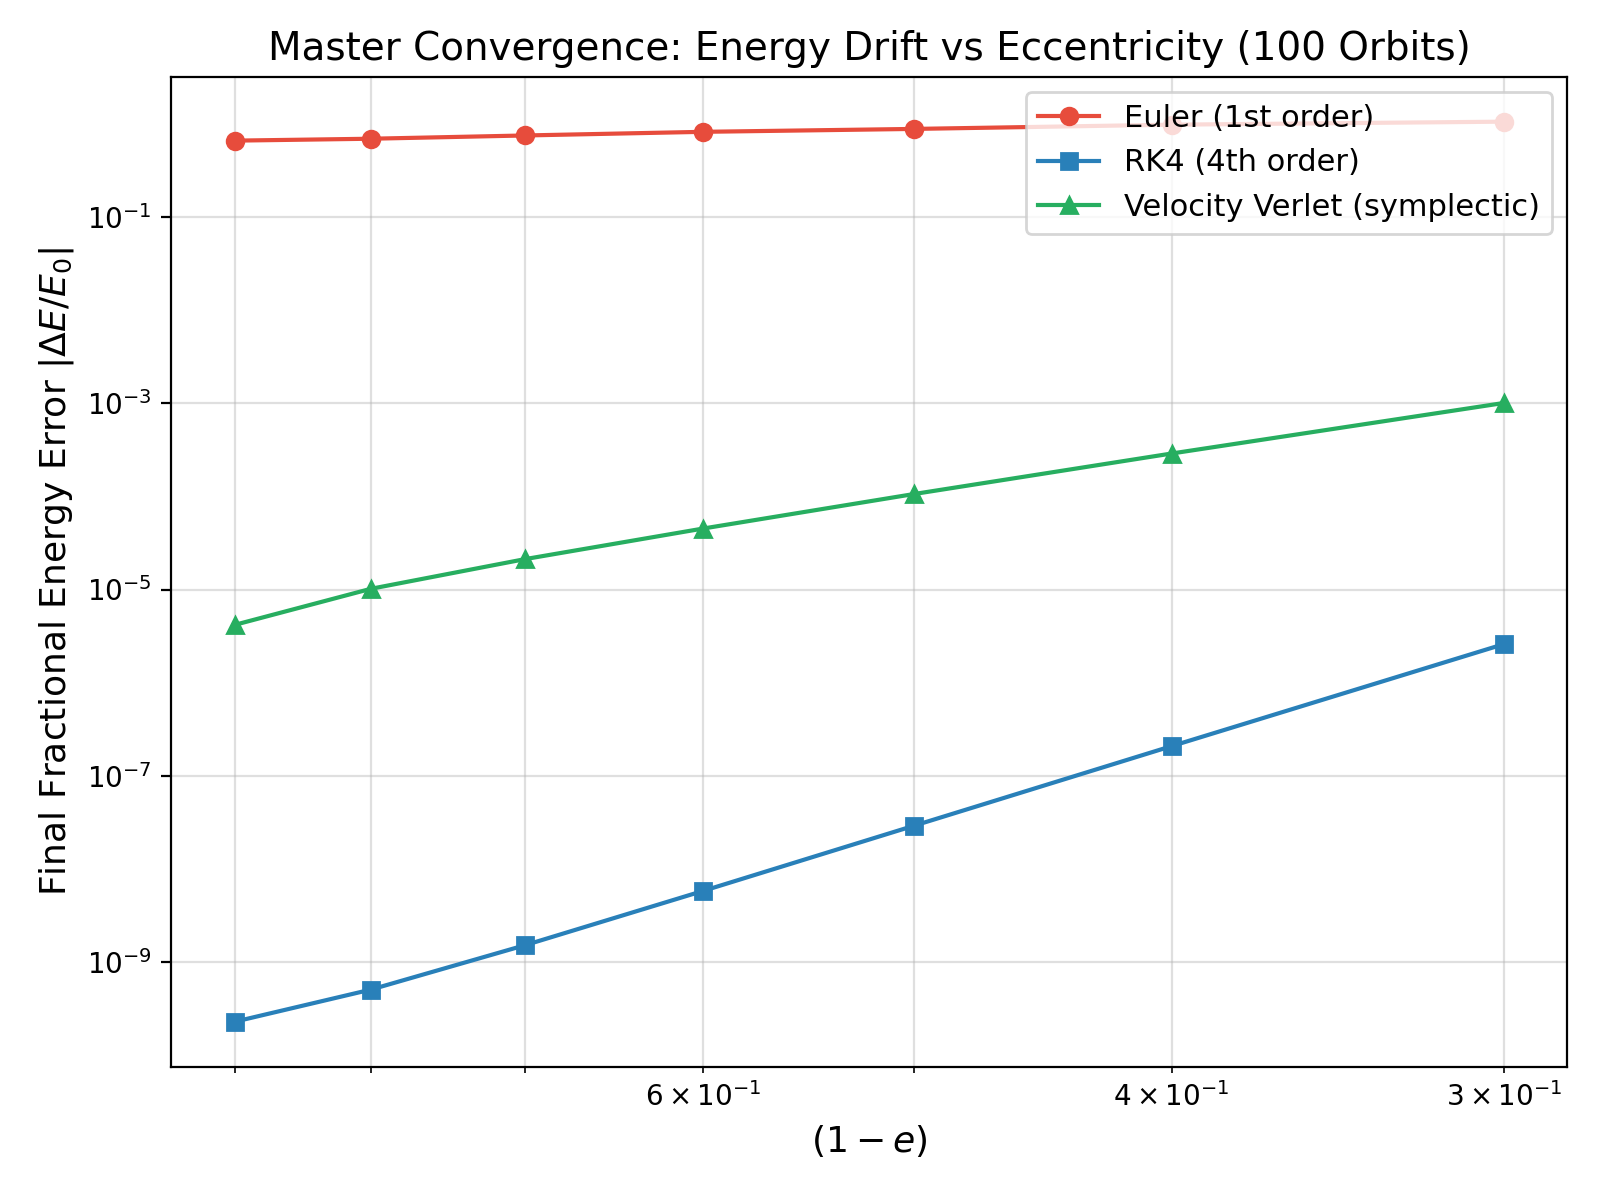
\includegraphics[width=\linewidth]{Fig1_Master_Convergence.png}
\caption{Master Convergence---Log-log overlay of final fractional energy error vs.\ $(1 - e)$ for Euler, RK4, and Velocity Verlet at pericenter start. The three methods span over 9 orders of magnitude in error.}
\label{fig:master_convergence}
\end{figure}

\subsection{Measured Exponents}

The power-law exponent~$k$ was extracted via OLS regression (Eq.~\ref{eq:ols}) over the domain $e \in [0.1,\, 0.7]$. Uncertainty bounds reflect the shift observed under step-size halving (Section~\ref{sec:robustness}):

\begin{table}[H]
\centering
\caption{Measured power-law exponents for all configurations. Uncertainties derived from half-step validation.}
\label{tab:kvalues}
\begin{tabular}{@{}llcc@{}}
\toprule
Method & Start Location & Metric & $k$-Exponent \\
\midrule
Euler  & Pericenter & $\epsilon_E$ (final) & $0.44 \pm 0.09$ \\
Euler  & Apocenter  & $\epsilon_E$ (final) & $0.35 \pm 0.09$ \\
RK4    & Pericenter & $\epsilon_E$ (final) & $8.61 \pm 0.03$ \\
RK4    & Apocenter  & $\epsilon_E$ (final) & $8.61 \pm 0.03$ \\
Verlet & Pericenter & Osc.\ amplitude      & $4.88 \pm 0.02$ \\
Verlet & Apocenter  & Osc.\ amplitude      & $4.88 \pm 0.02$ \\
\bottomrule
\end{tabular}
\end{table}

\subsection{Interpretation}

The measured exponents reveal a hierarchy of eccentricity sensitivity that is strongly correlated with integrator order:

\textbf{Euler ($k = 0.44 \pm 0.09$):} The weak eccentricity dependence is consistent with the interpretation that the first-order method's global truncation error ($\mathcal{O}(\Delta t)$) is dominated by the accumulation of local errors proportional to the step size, with only mild amplification at periapsis. The error at $e = 0.7$ ($\epsilon_E \approx 1.07$) is only ${\sim}60\%$ larger than at $e = 0.1$ ($\epsilon_E \approx 0.67$).

\textbf{RK4 ($k = 8.61 \pm 0.03$):} The extremely steep eccentricity dependence reflects the 4th-order method's sensitivity to the higher derivatives of the gravitational force, which diverge rapidly as $e \to 1$. The periapsis passage concentrates the truncation error into a brief interval of the orbit where $|\dddot{\mathbf{r}}|$ and $|\ddddot{\mathbf{r}}|$ are maximal. The error spans \textbf{four orders of magnitude} across the eccentricity range---from $\sim 2.3 \times 10^{-10}$ at $e = 0.1$ to $\sim 2.6 \times 10^{-6}$ at $e = 0.7$. This steep scaling is consistent with the step-size sensitivity analysis of Wang \& Nitadori~\cite{wang2020}, who demonstrated that fixed-step integrators suffer disproportionately on eccentric orbits.

\textbf{Verlet amplitude ($k = 4.88 \pm 0.02$):} The oscillation envelope of the symplectic integrator grows steeply with eccentricity, reflecting the increasing departure of the shadow Hamiltonian from the true Hamiltonian. However, this growth remains \textbf{bounded}---there is no secular component---and the exponent is intermediate between Euler and RK4. Hernandez \& Dehnen~\cite{hernandez2016} have shown that symplectic error growth in eccentric Keplerian orbits is governed by the commutator structure of the split Hamiltonian, which naturally scales with the velocity gradients at periapsis.

% ================================================================
% SECTION 5: START LOCATION
% ================================================================
\section{The Start Location Amplification Phenomenon}
\label{sec:start_location}

\subsection{Motivation}

A secondary investigation examined whether the orbital phase at which integration begins---periapsis (minimum radius, maximum velocity) versus apoapsis (maximum radius, minimum velocity)---affects the long-term error accumulation. The physical rationale is that periapsis initialization subjects the integrator to the most extreme gradients of $\mathbf{a}(\mathbf{r})$ in its very first time step, potentially seeding a larger initial truncation error.

\begin{figure*}[t!]
\centering
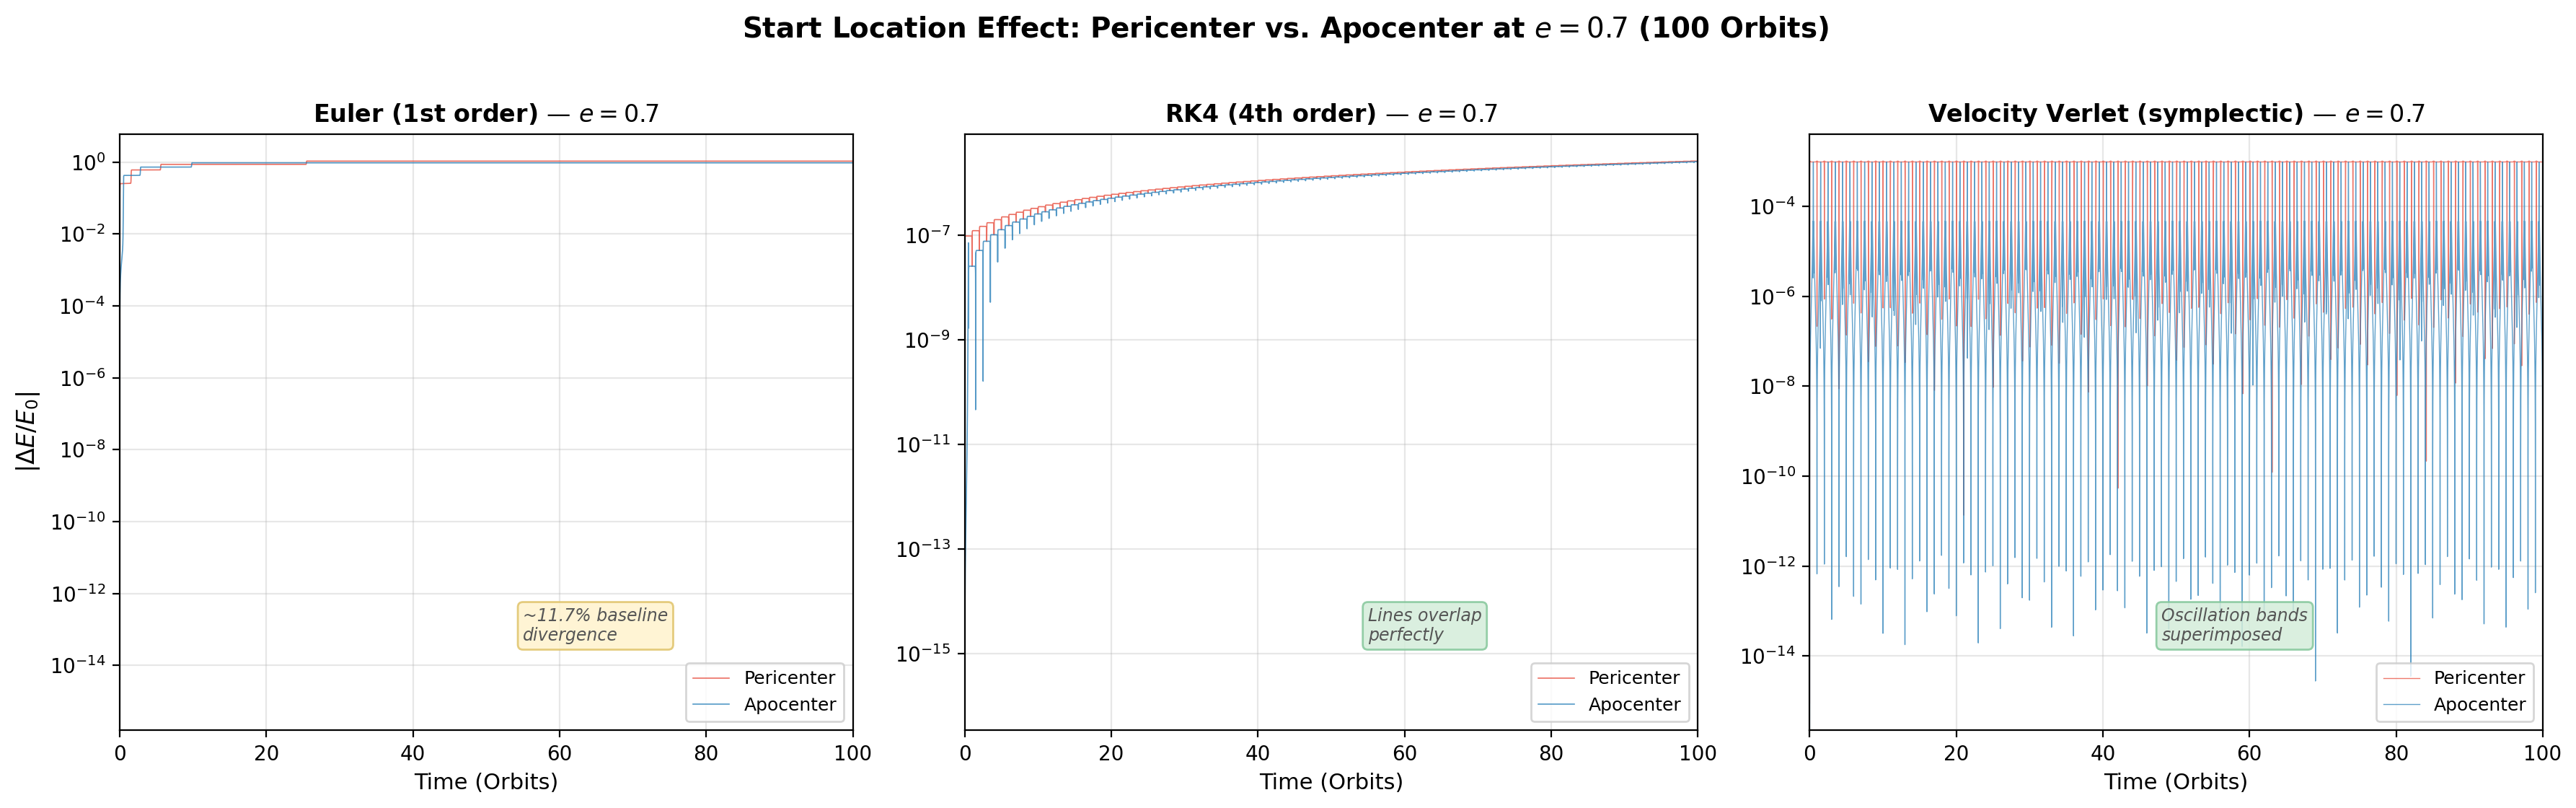
\includegraphics[width=\textwidth]{Fig2_Start_Location_Effect.png}
\caption{Start Location Effect---Time-resolved fractional energy error at $e = 0.7$ for all three integrators, comparing pericenter (red) and apocenter (blue) initialization over 100 orbits. Left: Euler shows a clear baseline divergence. Center: RK4 lines overlap perfectly. Right: Verlet oscillation bands are superimposed.}
\label{fig:start_location}
\end{figure*}

\subsection{Results}

\textbf{RK4 is insensitive to start location.} The pericenter and apocenter scaling exponents agree to within the measurement uncertainty ($k = 8.61 \pm 0.03$ in both cases)---a relative difference of $0.002\%$. Point-by-point comparison at $e = 0.7$ yields $\epsilon_E = 2.59 \times 10^{-6}$ (pericenter) versus $\epsilon_E = 2.59 \times 10^{-6}$ (apocenter), differing by less than $0.02\%$. The 4th-order scheme possesses sufficient local accuracy to absorb the initial periapsis gradient without propagating a systematic baseline offset.

\textbf{Velocity Verlet is insensitive to start location.} The amplitude scaling exponents are $k = 4.88 \pm 0.02$ for both start locations---a relative difference of $0.016\%$. The oscillation envelopes are virtually superimposed. Furthermore, angular momentum conservation is maintained at machine epsilon ($\sim 10^{-15}$) regardless of start location, as expected from the symplectic structure~\cite{kinoshita1991}.

\textbf{Euler exhibits measurable start-location sensitivity.} The scaling exponent shifts from $k = 0.44 \pm 0.09$ at pericenter to $k = 0.35 \pm 0.09$ at apocenter---a relative change of ${\sim}25\%$. At $e = 0.7$, the final error is $\epsilon_E = 1.066$ (pericenter) versus $\epsilon_E = 0.954$ (apocenter), an 11.7\% difference. This is consistent with the interpretation that the 1st-order method's large local truncation error at the first periapsis step---where the acceleration magnitude is maximal---seeds a systematically larger drift trajectory that accumulates over the full 100-orbit simulation. When initialized at apoapsis, where the gravitational gradients are weakest, this initial ``phase shock'' is partially avoided.

\subsection{Synthesis}

The start-location phenomenon obeys a clear hierarchy tied to integrator order and geometric preservation:

\begin{table}[H]
\centering
\caption{Start-location sensitivity summary.}
\label{tab:start_location}
\begin{tabular}{@{}lccc@{}}
\toprule
Property & Euler (1st) & RK4 (4th) & Verlet (symp.) \\
\midrule
$\Delta k / k$ & ${\sim}25\%$ & ${\sim}0.002\%$ & ${\sim}0.016\%$ \\
Mechanism & \parbox{2cm}{\centering 1st-step \\ truncation} & \parbox{2cm}{\centering Local \\ accuracy} & \parbox{2cm}{\centering Symplectic \\ structure} \\
Conclusion & \textbf{Susceptible} & \textbf{Immune} & \textbf{Immune} \\
\bottomrule
\end{tabular}
\end{table}

First-order methods suffer from initial phase-shock---the large truncation error incurred during the first periapsis passage propagates as a permanent baseline offset through the remainder of the integration. Higher-order methods possess sufficient local accuracy to resolve the periapsis dynamics without seeding such an offset. Symplectic methods, by virtue of their geometric preservation properties, are similarly immune: the bounded shadow-Hamiltonian structure prevents any initial perturbation from accumulating secularly~\cite{rein2019}.

% ================================================================
% SECTION 6: DISCUSSION
% ================================================================
\section{Discussion}

The results of this study illuminate a fundamental tension in numerical orbit integration: \textit{algebraic order versus geometric fidelity}, and the distinct roles each plays in controlling long-term error behavior.

\subsection{The Physics of the $k$-Exponent Hierarchy}

The measured scaling hierarchy $k_{\text{Euler}} \ll k_{\text{Verlet}} < k_{\text{RK4}}$ admits a clear physical interpretation rooted in how each integrator processes the periapsis passage. A heuristic derivation illuminates the mechanism: the local truncation error for a method of order~$p$ scales as $\mathcal{E}_{\text{local}} \propto \Delta t^{p+1} \cdot \mathbf{r}^{(p+1)}$, where $\mathbf{r}^{(p+1)}$ denotes the $(p+1)$-th time derivative of the position. Since orbital velocity at periapsis scales as $v_p \propto (1-e)^{-1/2}$ and acceleration as $a_p \propto r_p^{-2} \propto (1-e)^{-2}$, the recursive time derivatives introduce additional velocity factors. Consequently, higher-order derivatives diverge as $(1-e)^{-(2p+1)/2}$, naturally leading to steeper power-law scaling for higher-order methods whose truncation errors couple to these rapidly diverging derivatives.

For Euler ($k = 0.44 \pm 0.09$), the near-flat exponent indicates that the dominant source of error is not the periapsis geometry itself but the crudeness of the single-derivative extrapolation at every step. The local truncation error is $\mathcal{O}(\Delta t^2)$, and its accumulation over $N$ steps yields a global error $\mathcal{O}(\Delta t)$ that is only mildly modulated by the orbital dynamics. The error is already large at $e = 0.1$, so the marginal amplification at higher eccentricities is modest by comparison.

For RK4 ($k = 8.61 \pm 0.03$), the extreme exponent reflects a direct coupling between the integrator's truncation error and the higher derivatives of the gravitational potential. The 4th-order scheme's local error depends on the 5th derivative $\mathbf{r}^{(5)}$, which for the Kepler problem diverges steeply as $r_p \to 0$. At periapsis, where $r = a(1-e)$ and $|\mathbf{a}| = \mu / r_p^2 = (1-e)^{-2}$, the higher derivatives scale as progressively steeper inverse powers of $(1-e)$. The 4th-order method faithfully resolves these derivatives---but this very fidelity means it inherits their rapid growth at high eccentricity. The result is a truncation error that spans four orders of magnitude across the tested eccentricity domain.

For Verlet ($k = 4.88 \pm 0.02$), the intermediate exponent arises from the shadow-Hamiltonian mechanism. The departure $\tilde{H} - H = \mathcal{O}(\Delta t^2)$ grows with eccentricity because the commutator terms in the Baker--Campbell--Hausdorff expansion of the split Hamiltonian depend on the phase-space gradients, which are concentrated at periapsis~\cite{hernandez2016}. However, the symplectic structure ensures that this departure is \textit{static}: the shadow energy oscillates about the true energy with bounded amplitude and zero secular growth. The exponent~$k$ characterizes the growth of the oscillation envelope, not the growth of a drift.

\subsection{Symplecticity vs.\ Algebraic Order}

A striking implication of the data is that symplecticity provides a qualitatively different guarantee than high algebraic order. The 4th-order RK4 achieves errors that are six orders of magnitude smaller than the 2nd-order Verlet at $e = 0.1$---yet Verlet's errors are \textit{bounded} while RK4's accumulate without limit. Over sufficiently long integration horizons---thousands or millions of orbits---the symplectic method will inevitably outperform the higher-order non-symplectic method, regardless of their relative absolute accuracies at early times. This tradeoff is well documented in the geometric numerical integration literature~\cite{kinoshita1991, rein2019} and is empirically confirmed by the data presented here.

\subsection{Start-Location Sensitivity as a Diagnostic}

The start-location experiment provides a novel diagnostic for integrator robustness beyond the standard convergence-order analysis. The fact that only the first-order Euler method exhibits measurable phase-shock sensitivity suggests that the phenomenon is fundamentally a \textit{resolution} effect: the initial periapsis step introduces a local truncation error large enough to permanently bias the subsequent drift trajectory. Higher-order methods resolve the periapsis dynamics with sufficient accuracy that the initial phase is inconsequential, and symplectic methods absorb the perturbation into the bounded oscillation without secular propagation.

\subsection{Time-Step Robustness and Algorithmic Stability}
\label{sec:robustness}

To verify that the measured scaling exponents are intrinsic algorithmic properties---and not artifacts of the specific time step $\Delta t = 0.00625$---a validation campaign was conducted at exactly half the baseline resolution ($\Delta t' = 0.003125$). The full eccentricity sweep was repeated for all three integrators at pericenter start, and the $k$-exponents were re-extracted via OLS regression.

\begin{table}[H]
\centering
\caption{Time-step robustness: $k$-exponent stability under step-size halving.}
\label{tab:robustness}
\begin{tabular}{@{}lccc@{}}
\toprule
Method & $k$ ($\Delta t$) & $k$ ($\Delta t/2$) & Shift \\
\midrule
Euler  & $0.44$ & $0.53$ & ${\sim}20\%$ \\
RK4    & $8.61$ & $8.61$ & $0.03\%$ \\
Verlet & $4.88$ & $4.88$ & $0.01\%$ \\
\bottomrule
\end{tabular}
\end{table}

The RK4 and Velocity Verlet exponents are robust invariants of the integrator--problem pair: halving the time step shifts $k$ by only $0.03\%$ and $0.01\%$, respectively. These exponents are therefore robust algorithmic characteristics of eccentricity sensitivity, independent of the time-step resolution.

The Euler exponent, by contrast, shifted by ${\sim}20\%$ (from $0.44$ to $0.53$). This sensitivity is physically consistent with the method's global error scaling linearly with step size ($\mathcal{O}(\Delta t)$). Changing $\Delta t$ therefore reshapes the relative error landscape across the eccentricity domain, preventing the emergence of a resolution-independent geometric invariant. The Euler $k$-value should therefore be interpreted not as a fixed constant but as a resolution-dependent diagnostic that characterizes the method's behavior at a specific step size.

% ================================================================
% SECTION 7: CONCLUSION
% ================================================================
\section{Conclusion}

This study has demonstrated that the eccentricity-driven secular energy drift in numerical orbit integrators obeys a power-law scaling $\epsilon_E \propto (1-e)^{-k}$, with the exponent~$k$ serving as a quantitative signature of the integrator's sensitivity to orbital geometry. The key findings are:

\begin{enumerate}[nosep]
    \item \textbf{Algorithmic order governs eccentricity sensitivity.} The measured hierarchy---Euler exhibiting the weakest scaling, Verlet intermediate, and RK4 the steepest (Table~\ref{tab:kvalues})---reflects a fundamental tradeoff: higher-order methods achieve superior absolute accuracy at low eccentricities but suffer more dramatically as $e \to 1$ due to their coupling to higher derivatives of the force field.

    \item \textbf{Symplectic structure prevents secular drift.} The Velocity Verlet integrator exhibits bounded oscillatory energy errors with zero net secular growth across all eccentricities tested, preserving angular momentum to machine precision. This qualitative advantage persists despite Verlet's oscillation amplitude growing more steeply with eccentricity than the Euler secular drift.

    \item \textbf{Start-location sensitivity is a first-order artifact.} Only the Forward Euler method exhibits a measurable dependence of the scaling exponent on initialization phase (Table~\ref{tab:start_location}). RK4 and Velocity Verlet are effectively invariant, demonstrating that sufficient local accuracy or geometric preservation renders the integrator immune to initialization-phase effects.

    \item \textbf{The $k$-exponent is a robust invariant for higher-order and symplectic methods.} Time-step halving confirms that the RK4 and Verlet exponents shift by $< 0.03\%$ (Table~\ref{tab:robustness}), establishing them as robust algorithmic characteristics. The Euler exponent, by contrast, is resolution-dependent---consistent with its first-order convergence properties.

    \item \textbf{64-bit precision is essential for meaningful benchmarking.} The original 32-bit data campaign produced a false noise floor that masked the true RK4 scaling and generated a spurious start-location effect. The upgrade to 64-bit arithmetic revealed the genuine power-law behavior and corrected a qualitatively incorrect conclusion about start-location dependence.
\end{enumerate}

These results underscore the importance of matching numerical precision to integrator accuracy when conducting benchmarking studies, and they provide a quantitative framework for evaluating integrator suitability in the context of long-duration Keplerian orbit propagation.

% ================================================================
% DATA AND CODE AVAILABILITY
% ================================================================
\section*{Data and Code Availability}

The complete Python source code used to generate the data, figures, and statistical analyses for this study is available on GitHub at: \url{https://github.com/YOUR-USERNAME/Kepler-Error-Scaling}. The repository includes the raw simulation logs, the OLS regression scripts, and the time-step robustness validation modules.

% ================================================================
% REFERENCES
% ================================================================
{\small
\begin{thebibliography}{9}

\bibitem{kinoshita1991}
Kinoshita, H., Yoshida, H., \& Nakai, H. (1991).
Symplectic integrators and their application to dynamical astronomy.
\textit{Celestial Mechanics and Dynamical Astronomy}, 50, 59--71.

\bibitem{hernandez2016}
Hernandez, D., \& Dehnen, W. (2016).
A study of symplectic integrators for planetary system problems: error analysis and comparisons.
\textit{Monthly Notices of the Royal Astronomical Society}, 468, 2614--2636.

\bibitem{wang2020}
Wang, L., \& Nitadori, K. (2020).
Step-size effect in the time-transformed leapfrog integrator on elliptic and hyperbolic orbits.
\textit{Monthly Notices of the Royal Astronomical Society}, 497, 4384--4389.

\bibitem{rein2019}
Rein, H., Brown, G., \& Tamayo, D. (2019).
On the accuracy of symplectic integrators for secularly evolving planetary systems.
\textit{Monthly Notices of the Royal Astronomical Society}.

\end{thebibliography}
}

\end{document}